\documentclass{scrartcl}


\usepackage[english]{babel} 

\usepackage{amsfonts}
\usepackage{amsmath,amsthm,amssymb,upref}
\usepackage{tikz}
\usepackage[left=1cm, right = 1cm, top = 1cm, bottom = 1cm]{geometry}


\newtheorem{lemma}{Lemma}
\theoremstyle{definition}
\newtheorem{definition}{Definition}
\theoremstyle{remark}
\newtheorem{remark}{Remark}

\newcommand{\Frechet}{Fr\'echet }
\newcommand{\T}{\mathcal T}
\newcommand{\eps}{\varepsilon}
\newcommand{\N}{\mathbb N}
\newcommand{\R}{\mathbb R}
\newcommand{\Q}{\mathbb Q}

\newcommand{\del}{\partial}
\newcommand{\dist}{\operatorname{dist}}
\usetikzlibrary{calc}
\begin{document}


% IMPORTANT: a^2+c^2 = b^2 (sorry for that)
% AND: b > c > a

% Set a, b, c according to the rules above,
% set "padding factor" y to something arbitrary >= 0, e.g. 0.3
% don't touch x
\section{Right Triangles}
\begin{tikzpicture}
\pgfmathsetmacro{\a}{4}
\pgfmathsetmacro{\b}{5}
\pgfmathsetmacro{\c}{3}
\pgfmathsetmacro{\x}{\a + \b}
\pgfmathsetmacro{\y}{0.5}
\draw (0,0) -- node [below]{a}(\a,0) -- node[right]{c} (\a, \c) -- node[above]{b} (0,0);
\draw (-\x -\y +\a+ \b, 0) arc (180:90:\x + \y - \b) arc (90:atan(\c/\a):\x+\y-\b-\c) arc (atan(\c/\a):0:{\x+\y  -\c}) arc (0:-90:\x+\y-\a-\c) arc (-90:-90-atan(\a/\c):\x+\y-\a) arc (-90-atan(\a/\c):-180:\x+\y-\a-\b);
\end{tikzpicture}
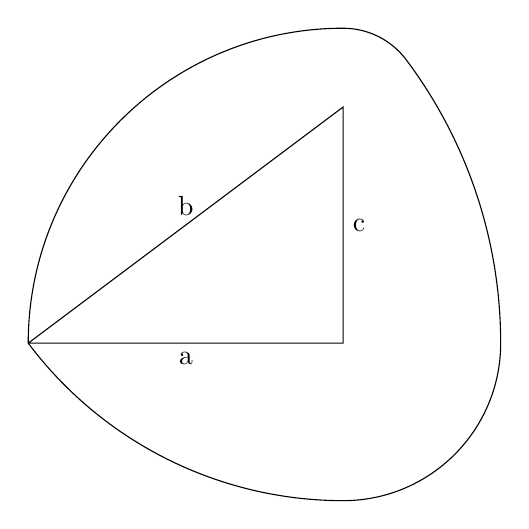
\begin{tikzpicture}
\pgfmathsetmacro{\a}{4}
\pgfmathsetmacro{\b}{5}
\pgfmathsetmacro{\c}{3}
\pgfmathsetmacro{\x}{\a + \b}
\pgfmathsetmacro{\y}{0.0}
\draw (0,0) -- node [below]{a}(\a,0) -- node[right]{c} (\a, \c) -- node[above]{b} (0,0);
\draw (-\x -\y +\a+ \b, 0) arc (180:90:\x + \y - \b) arc (90:atan(\c/\a):\x+\y-\b-\c) arc (atan(\c/\a):0:{\x+\y  -\c}) arc (0:-90:\x+\y-\a-\c) arc (-90:-90-atan(\a/\c):\x+\y-\a) arc (-90-atan(\a/\c):-180:\x+\y-\a-\b);
\end{tikzpicture}

\begin{tikzpicture}[scale=.4]
\pgfmathsetmacro{\a}{12}
\pgfmathsetmacro{\b}{13}
\pgfmathsetmacro{\c}{5}
\pgfmathsetmacro{\x}{\a + \b}
\pgfmathsetmacro{\y}{1}
\draw (0,0) -- node [below]{a}(\a,0) -- node[right]{c} (\a, \c) -- node[above]{b} (0,0);
\draw (-\x -\y +\a+ \b, 0) arc (180:90:\x + \y - \b) arc (90:atan(\c/\a):\x+\y-\b-\c) arc (atan(\c/\a):0:{\x+\y  -\c}) arc (0:-90:\x+\y-\a-\c) arc (-90:-90-atan(\a/\c):\x+\y-\a) arc (-90-atan(\a/\c):-180:\x+\y-\a-\b);
\end{tikzpicture}
\section{General Triangles}

% HERE: a > b > c
\begin{tikzpicture}[scale = 1.5]
\pgfmathsetmacro{\a}{4} % Change me
\pgfmathsetmacro{\b}{3} % Change me
\pgfmathsetmacro{\c}{2} % Change me
\pgfmathsetmacro{\y}{0.3} % Change me (>=0)
\pgfmathsetmacro{\temp}{\a*\a+\b*\b - \c*\c}
\pgfmathsetmacro{\d}{\temp/(2*\a)}
\pgfmathsetmacro{\h}{sqrt(\b*\b - \d * \d)}
\pgfmathsetmacro{\o}{acos((\b*\b + \c*\c - \a*\a)/(2* \b * \c))}
\pgfmathsetmacro{\p}{acos((-\b*\b + \c*\c + \a*\a)/(2* \a * \c))}
\pgfmathsetmacro{\q}{acos((\b*\b - \c*\c + \a*\a)/(2* \b * \a))}
\draw (0,0) -- node[below]{a} (\a, 0) -- node[right]{c} (\d, \h) -- node[above]{b} (0,0);
\draw (- \y, 0) arc (180:180-\p:\a+\y) arc (180-\p:\q:\a-\c+\y) arc (\q:0:\a+\b-\c+\y) arc (0:-\p:\b-\c+\y) arc (-\p:-180+\q:\b+\y) arc (-180+\q:-180:\y);
\end{tikzpicture}
\begin{tikzpicture}[scale = 1.5]
\pgfmathsetmacro{\a}{4} % Change me
\pgfmathsetmacro{\b}{3} % Change me
\pgfmathsetmacro{\c}{2} % Change me
\pgfmathsetmacro{\y}{0.0} % Change me (>=0)
\pgfmathsetmacro{\temp}{\a*\a+\b*\b - \c*\c}
\pgfmathsetmacro{\d}{\temp/(2*\a)}
\pgfmathsetmacro{\h}{sqrt(\b*\b - \d * \d)}
\pgfmathsetmacro{\o}{acos((\b*\b + \c*\c - \a*\a)/(2* \b * \c))}
\pgfmathsetmacro{\p}{acos((-\b*\b + \c*\c + \a*\a)/(2* \a * \c))}
\pgfmathsetmacro{\q}{acos((\b*\b - \c*\c + \a*\a)/(2* \b * \a))}
\draw (0,0) -- node[below]{a} (\a, 0) -- node[right]{c} (\d, \h) -- node[above]{b} (0,0);
\draw (- \y, 0) arc (180:180-\p:\a+\y) arc (180-\p:\q:\a-\c+\y) arc (\q:0:\a+\b-\c+\y) arc (0:-\p:\b-\c+\y) arc (-\p:-180+\q:\b+\y) arc (-180+\q:-180:\y);
\end{tikzpicture}


% HERE: a > b > c
\begin{tikzpicture}[scale = 1.5]
\pgfmathsetmacro{\a}{4} % Change me
\pgfmathsetmacro{\b}{3} % Change me
\pgfmathsetmacro{\c}{2} % Change me
\pgfmathsetmacro{\y}{0.0} % Change me (>=0)
\pgfmathsetmacro{\temp}{\a*\a+\b*\b - \c*\c}
\pgfmathsetmacro{\d}{\temp/(2*\a)}
\pgfmathsetmacro{\h}{sqrt(\b*\b - \d * \d)}
\pgfmathsetmacro{\o}{acos((\b*\b + \c*\c - \a*\a)/(2* \b * \c))}
\pgfmathsetmacro{\p}{acos((-\b*\b + \c*\c + \a*\a)/(2* \a * \c))}
\pgfmathsetmacro{\q}{acos((\b*\b - \c*\c + \a*\a)/(2* \b * \a))}
\draw (0,0) -- node[below]{a} (\a, 0) -- node[right]{c} (\d, \h) -- node[above]{b} (0,0);
\draw (- \y, 0) arc (180:180-\p:\a+\y) arc (180-\p:\q:\a-\c+\y) arc (\q:0:\a+\b-\c+\y) arc (0:-\p:\b-\c+\y) arc (-\p:-180+\q:\b+\y) arc (-180+\q:-180:\y);
\end{tikzpicture}
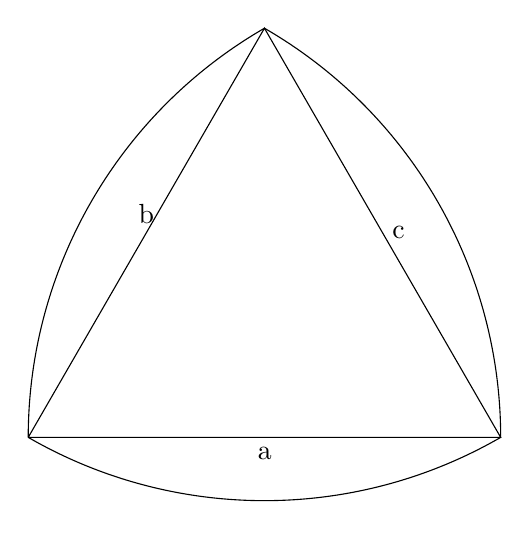
\begin{tikzpicture}[scale = 2]
\pgfmathsetmacro{\a}{3} % Change me
\pgfmathsetmacro{\b}{3} % Change me
\pgfmathsetmacro{\c}{3} % Change me
\pgfmathsetmacro{\y}{0.0} % Change me (>=0)
\pgfmathsetmacro{\temp}{\a*\a+\b*\b - \c*\c}
\pgfmathsetmacro{\d}{\temp/(2*\a)}
\pgfmathsetmacro{\h}{sqrt(\b*\b - \d * \d)}
\pgfmathsetmacro{\o}{acos((\b*\b + \c*\c - \a*\a)/(2* \b * \c))}
\pgfmathsetmacro{\p}{acos((-\b*\b + \c*\c + \a*\a)/(2* \a * \c))}
\pgfmathsetmacro{\q}{acos((\b*\b - \c*\c + \a*\a)/(2* \b * \a))}
\draw (0,0) -- node[below]{a} (\a, 0) -- node[right]{c} (\d, \h) -- node[above]{b} (0,0);
\draw (- \y, 0) arc (180:180-\p:\a+\y) arc (180-\p:\q:\a-\c+\y) arc (\q:0:\a+\b-\c+\y) arc (0:-\p:\b-\c+\y) arc (-\p:-180+\q:\b+\y) arc (-180+\q:-180:\y);
\end{tikzpicture}
\section{Comments}
The constant width of each shape is 
\[r = a + b - c + y\]
if $a > b > c$.

Construction follows "Mathematical Models - Henry Martyn Cundy (1961)".

\end{document}
